\chapter{AquaCrop scenario analysis for development of environment-specific agricultural management strategies}\label{ch:aquacropscen}
\chaptermark{Management scenario analysis}

\definecolor{bunds}{rgb}{0.74, 0.74, 0.74}
\definecolor{m50}{rgb}{0.53, 0.81, 0.92}
\definecolor{m95}{rgb}{0.28, 0.24, 0.55}
\definecolor{rest}{rgb}{0.55, 0.40, 0.03}
\definecolor{rwh}{rgb}{0.80, 0.41, 0.79}
\definecolor{tawm}{rgb}{1.00, 1.00, 0.00}
\definecolor{tawp}{rgb}{1.00, 0.55, 0.00}
\definecolor{w15}{rgb}{0.20, 0.80, 0.20}
\definecolor{w30}{rgb}{0.00, 0.39, 0.00}

This chapter is based on:\\
\longfullcite{vangaelen2013a}\\[6pt]
\&\\[6pt]
\longfullcite{vangaelen2014a}

\section{Introduction}
Due to the increasing world population and prosperity, global food production needs a 70\% increase by 2050 according to the Food and Agriculture Organization \parencite{fao2011}. To achieve this in a sustainable way by taking into account the limited land and water resources, an increase in productivity needs to be accompanied by an increase in crop water productivity. Improved agricultural management is one of the key solutions for upgrading (crop) water productivity. Particularly, in drought-prone regions where crop production is determined by variable rainfall, dry spells and droughts, rather than by low total rainfall, improved agricultural management shows great potential to upgrade crop water productivity \parencite{rockstrom2003c, wani2008a}.

Ample experimental research has been conducted to investigate the effect of agricultural management on crop (water) productivity. However, experimental research is time- and resource-consuming, certainly when several management options need to be evaluated. Moreover, the effect of agricultural management is strongly dependent on the complex interactions between rainfall pattern, soil characteristics and cropping system of a particular research site. Since experimental research results are affected by the specific experimental set-up, they can not be used to define general guidelines on efficient and sustainable agricultural management. By contrast, well calibrated crop models allow for very efficient and extensive scenario analysis. Moreover, they contribute to the understanding of interactions between environmental and management factors, facilitate long-term assessments with historical climate data, and enable assessment of future climate scenarios. All this makes them very suitable tools to assess crop response to agricultural management. 

Several simulation studies have been conducted to assess the effect of agronomic practices and water-saving techniques on crop production for irrigated or rainfed cropping systems using crop models such as APSIM \parencite[e.g.][]{akponikpe2010, kahinda2007}, CropSyst \parencite[e.g.][]{jalota2010, lehmann2013}, AquaCrop \parencite[e.g.][]{abrha2012, biazin2012, shrestha2013} and CERES \parencite[e.g.][]{he2012, rinaldi2004, timsina2008}. However, most of these studies evaluate agricultural management strategies for a specific case-study area, crop or cropping system whereby limited attention is paid to the interaction between management, crop and environmental factors. Also, most studies only consider a limited number of agricultural management options. Moreover, most simulation studies just assess the effect of different management scenarios on crop yield. Only few studies \parencite{arora2006, biazin2012,jalota2010, kahinda2007,shrestha2013, timsina2008} tend towards more sustainable decision making by assessing the effect on both yield and crop water productivity. 

This chapter presents a simulation approach to assess agricultural management strategies to optimize both crop yield and crop water productivity in rainfed cropping systems using the AquaCrop model \parencite{hsiao2009,steduto2009,raes2009a,vanuytrecht2014a}. With the goal to support development of environment-specific management guidelines, this simulation approach also intents to improve understanding of the interactions between management, soil, climate, and crop characteristics. An example scenario analysis for drought-prone rainfed cropping systems is conducted to assess the potential of the presented simulation approach and illustrate how simulation results can be analysed with special attention for management-environment interactions. 

\section{Simulation experiment}
A simulation experiment was set up to assess the effect of several agricultural management practices on \Y and \WPET for a wide range of rainfed cropping systems. By means of a factorial simulation experiment using the AquaCrop model, 10 agricultural management practices were studied for 81 different farming systems. 

\subsection{The AquaCrop model}
A test version of AquaCrop 4.0 (AquaCrop 4.0$^\ast$) was used for this simulation experiment. AquaCrop simulates crop productivity using a four-step process as discussed in \autoref{sec:ch2_ACsteps}. First, green crop canopy cover (\CC) is simulated. In a second step, crop transpiration (\Tr) is simulated considering reference evapotranspiration (\ETo) and a crop transpiration coefficient ($Kc_{Tr}$) that is proportional to the simulated canopy cover. Next, crop transpiration is converted into dry above-ground biomass production (\B). In a final step, crop biomass is converted to crop yield (\Y) by means of the harvest index (\HI). Crop yield per unit of water evapotranspired (\ET) is given by the ET crop water productivity (\WPET). During this four-step simulation process, the model accounts for the effect of various abiotic stresses, including water stress, temperature stress, soil salinity stress and soil fertility stress (\autoref{sec:ch2_abioticfac}). In addition, the effect of several agricultural management practices can be taken into account as discussed in \autoref{sec:ch2_Mgmt}. 

\subsection{Cropping systems}
By combining three different climatic conditions, crop varieties, soil types and soil fertility levels, 81 cropping systems were defined.
\begin{itemize}
\item \textbf{Climatic conditions}: Three different locations with varying climatic conditions were selected: Tunis (Tunisia), Mekelle (Ethiopia) and Chitedze (Malawi). \autoref{tab:ch5_locations} shows that these three locations cover the full range from semi-arid to sub-humid climatic conditions. 
\item \textbf{Crop variety}: Three barley (\textit{Hordeum vulgare} L.) varieties, with a typical growing cycle length of 90 days (short), 105 days (medium) and 120 days (long)\parencite{fao2007} were considered. Barley was selected as a crop because of its wide geographical distribution, its ability to grow in a wide variety of environments and its availability as calibrated crop in the AquaCrop database. All three varieties were simulated using the default AquaCrop parameters calibrated by \textcite{abrha2012}. Only the time to senescence and maturity was adapted because varieties differed in the length of the mid-season stage. Crop parameters describing crop response to soil fertility stress were calibrated with the automatic calibration procedure using the default settings: very strong \CCx reduction and medium canopy decline in the season for a relative biomass production (\Brel) of 50\%.
\item \textbf{Soil type}: Deep uniform soil profiles of three soil textural classes were considered: loamy sand, silt and clay loam. These textural classes were selected because they strongly differ in total available soil water (TAW), a major determinant of water availability to the crop. The default AquaCrop soil parameters for each soil textural class where used (\autoref{tab:ch5_soils}). Assuming that all soils are well structured, the default \Ksat value for the silt soil was increased from the default of \SI{50}{mm/d} to \SI{100}{mm/d} in order to avoid excessive surface runoff.
\item \textbf{Soil fertility level}: Three soil fertility levels, i.e. non limiting soil fertility (\Brel of 100\%), moderate soil fertility (\Brel of 60\%) and poor soil fertility (\Brel of 40\%) were selected to represent differences in fertilizer use between various farming systems.
\end{itemize}

\begin{table}[!ht]
\setlength{\tabcolsep}{4.3pt} %default is columnspace =6pt
 	\caption{Three selected locations with local average climatic conditions according to \textcite{fao2005}. The climate types are defined according to the Köppen-Geiger classification system \parencite{peel2007} in which B is dry (arid and semi-arid) climate, C is mild temperate climate, w is dry winter, S is steppe, a is hot summer, k is cold. The growing season is defined as the period in which rainfall exceeds 0.5 times the reference evapotranspiration (\ETo). The aridity index (AI) is the ratio of the annual rainfall and \ETo.\label{tab:ch5_locations}}
\begin{tabular}{lrrr}
\toprule
\textbf{Location} & \multicolumn{1}{c}{\textbf{Chitedze}} & \multicolumn{1}{c}{\textbf{Mekelle}} & \multicolumn{1}{c}{\textbf{Tunis}} \\
\midrule
Country  & \multicolumn{1}{c}{Malawi} & \multicolumn{1}{c}{Ethiopia} & \multicolumn{1}{c}{Tunisia} \\
Coordinates & \multicolumn{1}{c}{13.98°S, 33.63°E}& \multicolumn{1}{c}{13.5°N, 39.48°E}& \multicolumn{1}{c}{36.83°N, 10.13°E}\\
Altitude (m a.s.l.) & \multicolumn{1}{c}{1149} & \multicolumn{1}{c}{2070} & \multicolumn{1}{c}{4} \\
\midrule
\textbf{Climate} & \multicolumn{1}{l}{} & \multicolumn{1}{l}{} & \multicolumn{1}{l}{} \\
Type  & \multicolumn{1}{c}{Cwa} & \multicolumn{1}{c}{BSk} & \multicolumn{1}{c}{BSk} \\
Aridity  & \multicolumn{1}{c}{Sub-humid} & \multicolumn{1}{c}{Semi-arid} & \multicolumn{1}{c}{Semi-arid} \\
Rainfall regime & \multicolumn{1}{c}{monomodal} & \multicolumn{1}{c}{monomodal} & \multicolumn{1}{c}{monomodal} \\
Annual rainfall (\si{mm})& \multicolumn{1}{c}{923} & \multicolumn{1}{c}{620} & \multicolumn{1}{c}{436} \\
Annual \ETo (\si{mm})& \multicolumn{1}{c}{1349} & \multicolumn{1}{c}{1497} & \multicolumn{1}{c}{1093} \\
Annual AI (\si{mm/mm})& \multicolumn{1}{c}{0.68} & \multicolumn{1}{c}{0.41} & \multicolumn{1}{c}{0.4} \\
\midrule
\textbf{Growing season} & \multicolumn{1}{c}{} & \multicolumn{1}{c}{} & \multicolumn{1}{c}{} \\
Start & \multicolumn{1}{c}{November} & \multicolumn{1}{c}{June} & \multicolumn{1}{c}{October} \\
End   & \multicolumn{1}{c}{April} & \multicolumn{1}{c}{September} & \multicolumn{1}{c}{April} \\
Average length (d)  & \multicolumn{1}{c}{153} & \multicolumn{1}{c}{88} & \multicolumn{1}{c}{172} \\
\bottomrule
\end{tabular}%
  %
  \setlength{\tabcolsep}{6pt}
\end{table}

\begin{table}
	\centering
 	\caption{Three selected soil textural classes and the volumetric soil water content at wilting point (\Tpwp), field capacity (\Tfc) and saturation (\Tsat), total available soil water (TAW), saturated hydraulic conductivity (\Ksat) and surface runoff curve number (CN).\label{tab:ch5_soils}}
\begin{tabular}{lcccccc}
\toprule
\textbf{Soil Type} & \textbf{\Tpwp} & \textbf{\Tfc} & \textbf{\Tsat} & \textbf{TAW} & \textbf{\Ksat} & \textbf{CN} \\
\textbf{} & \textbf{(vol\%)} & \textbf{(vol\%)} & \textbf{(vol\%)} & \textbf{(\si{mm/m})} & \textbf{(\si{mm/d})} & \textbf{(-)} \\
\midrule
Loamy Sand & 8     & 16    & 38    & 80    & 800   & 65 \\
Silt  & 9     & 33    & 43    & 240   & 100   & 75 \\
Clay loam & 23    & 39    & 50    & 160   & 100   & 75 \\
\bottomrule
\end{tabular}%
\end{table}
\clearpage
\subsection{Agricultural management}
The effect of nine agricultural management practices was studied for each of the 81 cropping systems (\autoref{tab:ch5_mgmt}). In addition, a reference simulation served as a standard to evaluate the effectiveness of the different management practices. This reference simulation only considered soil fertility management but no additional management practices. 

Management practices like mulches, rainwater harvesting, and soil bunds are strategies that farmers implement to increase productivity beyond what is obtained under reference conditions. Other practices such as a restrictive soil layer and weed infestation are constraints under which farmers operate. Resolving these constraints might boost crop productivity. More detailed information on the required AquaCrop input, implementation and calculation procedures for the various agricultural management practices is presented in \autoref{ch:aquacrop}.

%\begin{table}[htbp]
\begin{tabularx}{\textwidth}{llX}
	\caption{Overview of different agricultural management practices that were evaluated for the 81 different cropping systems.\label{tab:ch5_mgmt}}\\
\toprule
\textbf{Management} & \textbf{Symbol} & \textbf{Description} \\
\midrule
Reference & Ref   & Only soil fertility management \\
Mulches & M50   & 50 \% evaporation reduction due to mulches \\
      & M95   & 95 \% evaporation reduction due to mulches \\
Field surface management & Bunds & Soil bunds of \SI{0.25}{m} \\
      & RWH   & Rainwater harvesting, runoff agriculture with 10:1 catchment-to-cropping area ratio \\
Soil management & Restr & Restrictive soil layer at \SI{0.5}{m} depth \\
      & TAW+  & TAW increased by \SI{50}{mm/m} \\
      & TAW-  & TAW decreased by \SI{50}{mm/m} \\
Weed management & W15   & 15\% relative weed cover, crop more competitive than weed \\
      & W30   & 30\% relative weed cover, crop more competitive than weed \\
\bottomrule
\end{tabularx}%
%\end{table}

\subsection{Simulation period, growing period and initial conditions}
The simulation period was determined by availability of weather data for each location. A total of 30 growing seasons was simulated for cropping systems in Chitedze (1980-2010) and Mekelle (1961-1973, 1981-1985, 1988, 1992-2002), while only 23 seasons were simulated (1979-2001) for cropping systems in Tunis. Simulations started each year at the end of the dry period on 1 October for Chitedze, 1 June for Mekelle, and 1 August for Tunis. At that moment the initial soil water content was assumed to be at permanent wilting point due to the high \ETo and limited rainfall in the dry period.

The first day of the growing period (sowing date) was automatically generated by AquaCrop based on a rainfall onset criteria of at least \SI{30}{mm} rainfall in a 5-day period for Chitedze and Mekelle and \SI{25}{mm} in a 5-day period for Tunis. Searching for fulfilment of the onset criteria was started at 1 June in Mekelle, and 1 October in Chitedze and Tunis. Since farmers would not sow immediately after the first rains, the second occurrence of the criteria fulfilment was accepted as a sowing date for Mekelle and Tunis. For Chitedze the third occurrence was accepted because of the very irregular start of the rainy season \parencite{scroyen2012}. If no appropriate sowing day was found before 31 January (Chitedze), 31 August (Mekelle) and 31 December (Tunis), the season was considered as a season with harvest failure (yield equal to \SI{0}{t/ha}) because of insufficient rainfall. 

\subsection{Impact analysis}
The effectiveness of each agricultural management practice was assessed by means of the \Y and \WPET response given by: 
\begin{equation}
 P_{response,m}=\dfrac{P_m-P_{ref}}{P_{ref}}\cdot 100
  \label{eq:ch5_response}
\end{equation}
where P$_{response,m}$ is the average response (\%) of productivity parameter \Y (\si{t/ha}) or \WPET (\si{kg/m^3}) to management practice m, P$_m$ and P$_{ref}$ is the average productivity (Y or \WPET) under certain environmental conditions with and without management practice m respectively. Response values express the relative increase (positive response values) or decrease (negative response values) of the average \Y and \WPET for certain environmental conditions due to a certain management strategy in comparison to the reference management. 

The \Y and \WPET response to all nine management practices was assessed for each cropping system. Furthermore, response values were analysed making a distinction between wet, dry and normal growing seasons for each location. Each of the 30 (Chitedze, Mekelle) or 23 (Tunis) simulated growing seasons was classified as dry, normal or wet based on a frequency analysis of seasonal rainfall with RAINBOW \parencite{raes2006a}. Seasonal rainfall was calculated as the sum of the daily rainfall from November to April (Chitedze), June to September (Mekelle) and October to April (Tunis). Growing seasons with seasonal rainfall with an exceedance probability of at least 70\% or less than 30\%, were classified as dry and wet respectively, whereas all others were classified as normal growing seasons. \autoref{tab:ch5_rainfall}, which shows the average seasonal rainfall for every seasonal rainfall class, indicates that the average seasonal rainfall in wet seasons in Mekelle was not significantly different from dry growing seasons in Chitedze. Similarly, normal and dry seasons in Mekelle did not differ significantly from the wet and normal growing seasons in Tunis respectively. 

\begin{table}
 	\caption{Seasonal rainfall classes for every location with the number of seasons (n), average seasonal rainfall, standard deviation (SD) and coefficient of variation (CV) over the simulation period. Values with the same subscript do not differ at a 0.05 significance level.}
\begin{tabular}{lccccc}
\toprule
\multicolumn{1}{l}{\textbf{Location }} & \multicolumn{1}{c}{\textbf{Seasonal rainfall}} & \multicolumn{4}{c}{\textbf{Seasonal rainfall }} \\
      & \multicolumn{1}{c}{\textbf{class}}  & \multicolumn{1}{l}{n} & \multicolumn{1}{l}{average (\si{mm})} & \multicolumn{1}{l}{SD (\si{mm})} & \multicolumn{1}{l}{CV (\%)} \\
\midrule
\multicolumn{1}{l}{Chitedze} & Wet   & 8     & 1077.5$_a$ & 89    & 8.3 \\
\multicolumn{1}{l}{} & Normal & 15    & 830.0$_b$  & 58.1  & 7 \\
\multicolumn{1}{l}{} & Dry   & 7     & 644.4$_c$ & 89.6  & 13.9 \\
\multicolumn{1}{l}{Mekelle} & Wet   & 12    & 652.5$_c$ & 113.1 & 17.3 \\
\multicolumn{1}{l}{} & Normal & 4     & 470.8$_d$ & 44.3  & 9.4 \\
\multicolumn{1}{l}{} & Dry   & 14    & 382.2$_e$ & 43.1  & 11.3 \\
\multicolumn{1}{l}{Tunis} & Wet   & 8     & 507.2$_d$ & 84.7  & 16.7 \\
\multicolumn{1}{l}{} & Normal & 8     & 355.6$_e$ & 50.2  & 14.1 \\
      & Dry   & 7     & 216.3$_f$ & 44.9  & 20.8 \\
\bottomrule
\end{tabular}%
  \label{tab:ch5_rainfall}%
\end{table}

Since the effectiveness of management practices was analysed on the basis of average \Y and \WPET values, it also includes seasons in which grain yield was zero. By contrast, the frequency of failure years is very decisive for adoption of a management strategy by risk averse farmers. For that reason, additional analysis of the frequency of harvest failure, i.e. percentage of seasons with \Y being \SI{0}{t/ha}, was conducted.

\section{Results}
The average \Y and \WPET response to the nine different agricultural management strategies is depicted in \autoref{fig:ch5_ScenClim} and represents the increase or decrease of the average \Y and \WPET over all simulated growing seasons and cropping systems (combinations of crop type, soil type and soil fertility level) due to the implementation of these strategies. In \autoref{fig:ch5_ScenClim} responses are presented for different weather conditions (combinations of a location and seasonal rainfall) ranging from very dry (dry growing seasons in Tunis) to more humid (wet growing seasons in Chitedze). No responses are presented for dry growing seasons in Tunis as insufficient rainfall resulted in complete failure of harvest for all those seasons. 

\begin{figure}[tbhp]
	\centering
		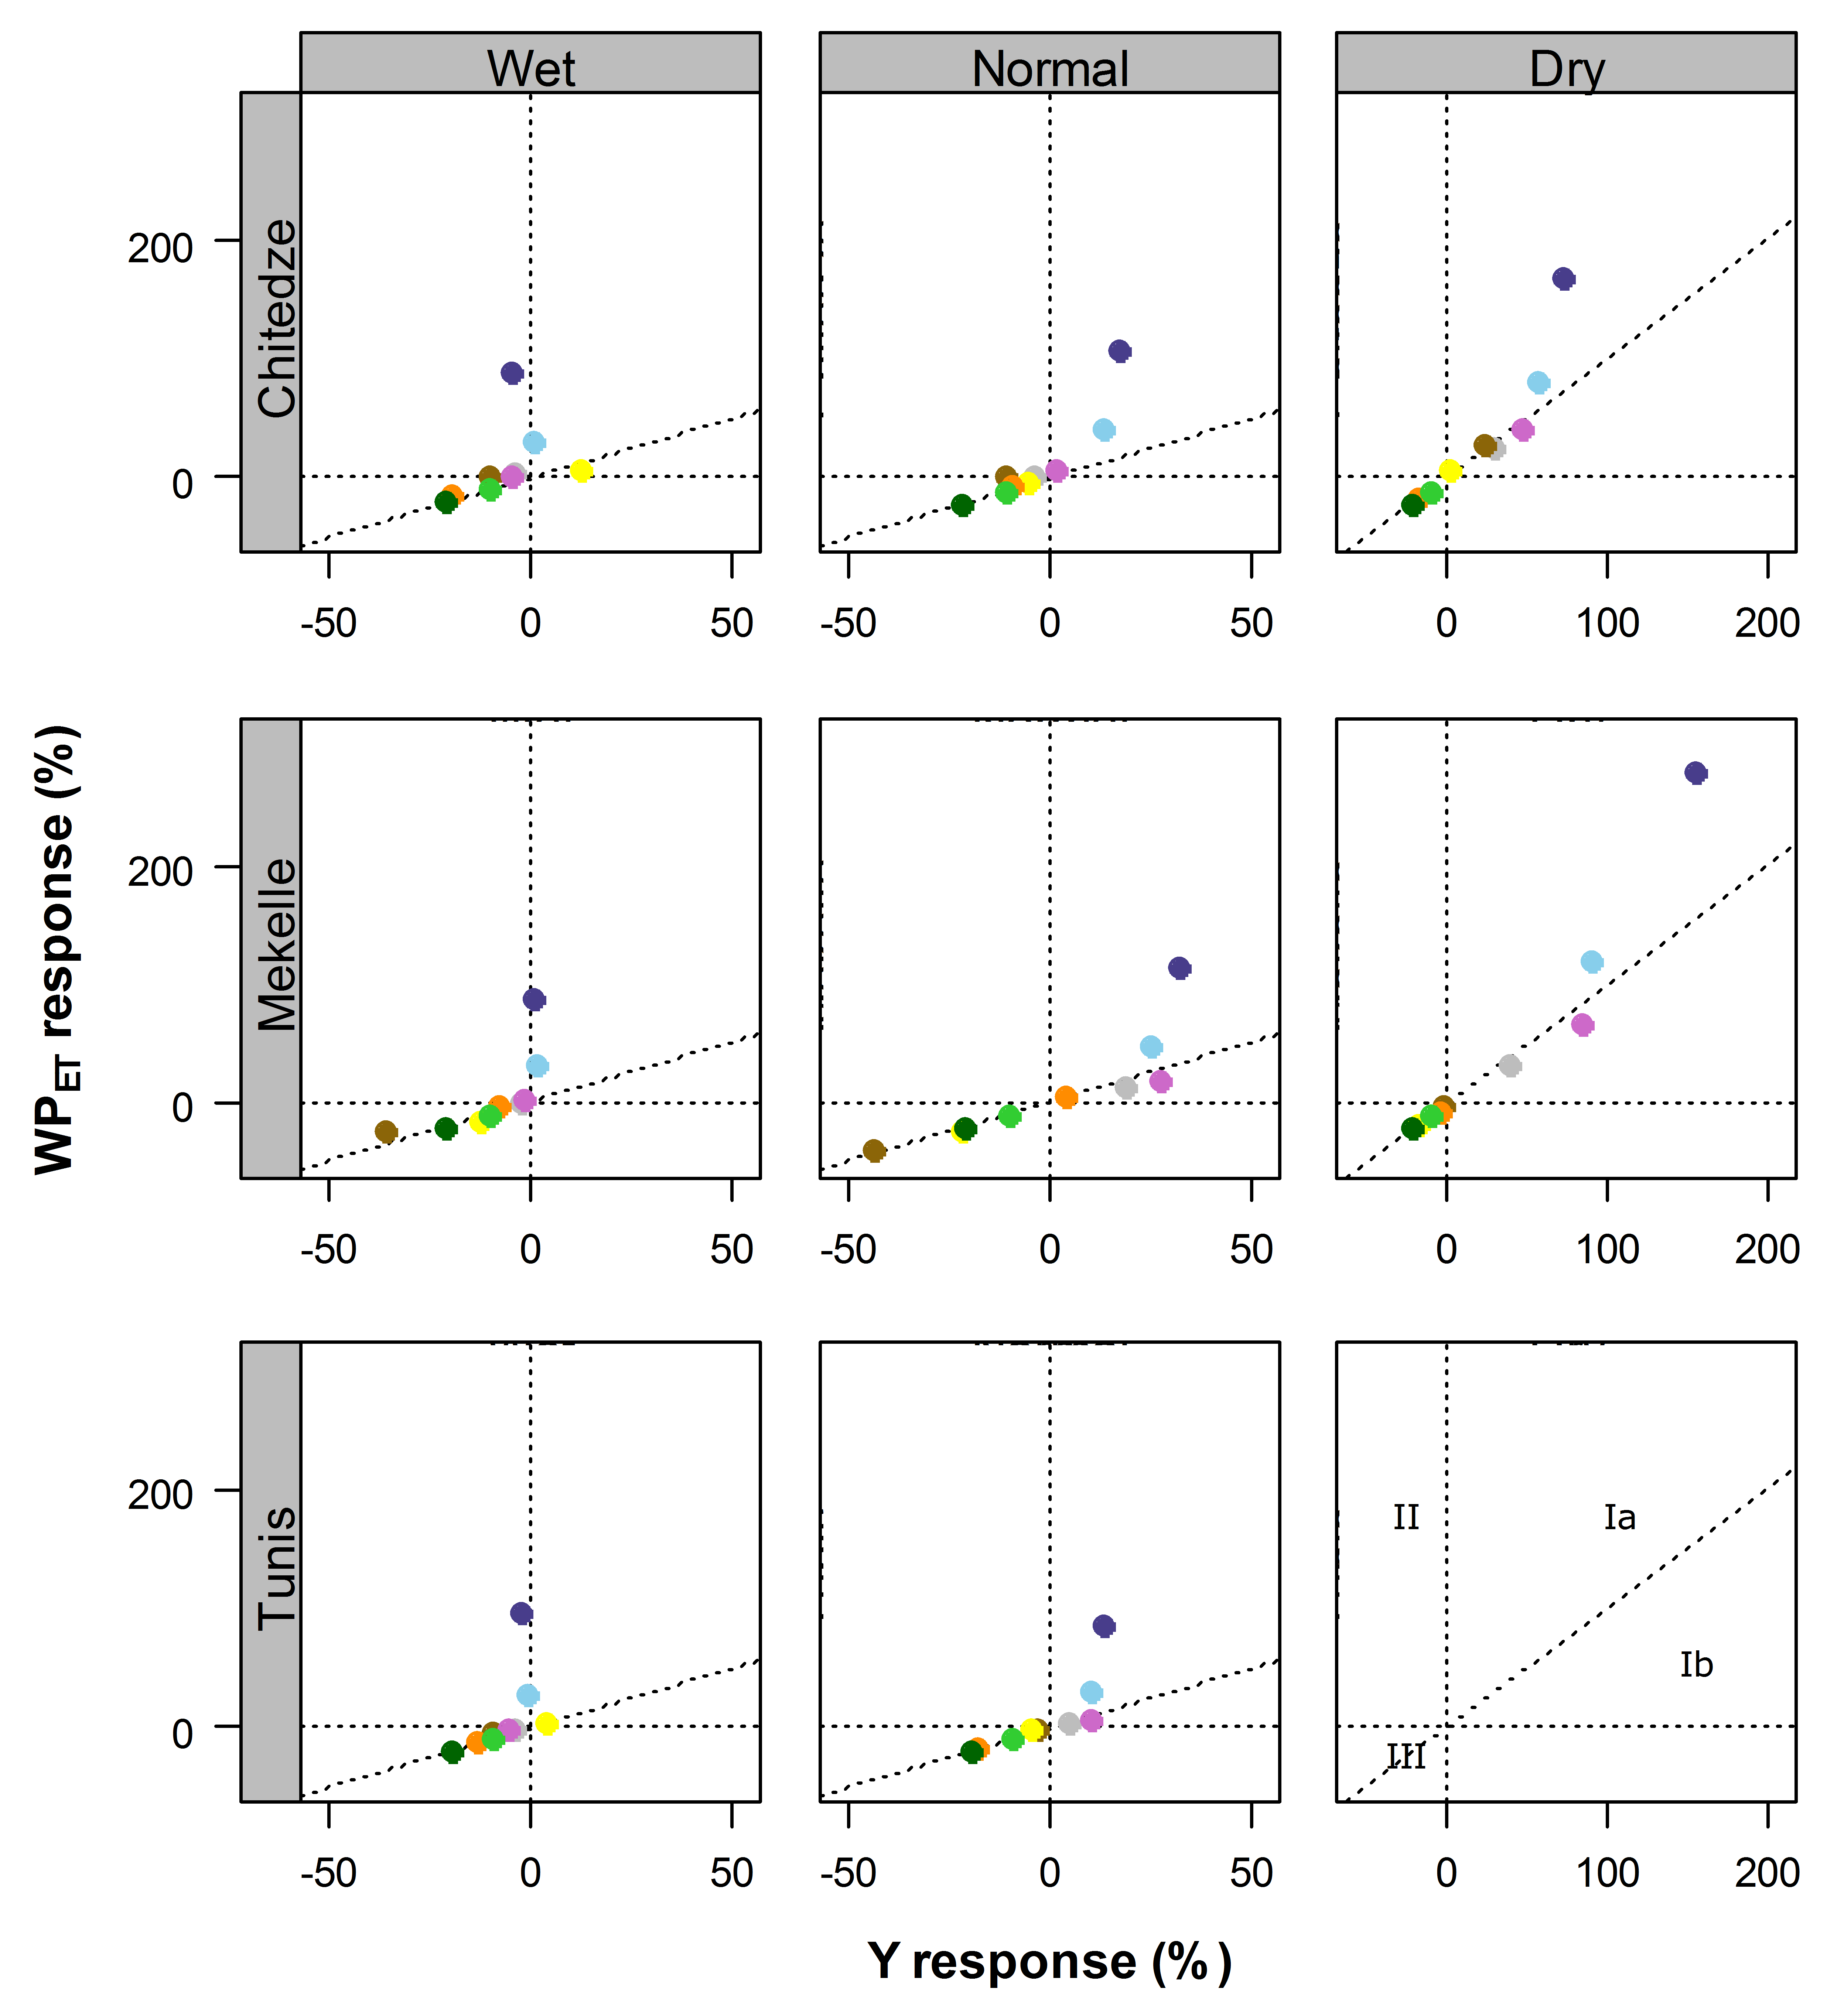
\includegraphics[width=\textwidth]{ScenClim_600dpi.png}
	\caption{Average yield (\Y) and crop water productivity (\WPET) response to different agricultural management strategies, i.e. \TAWm (\textcolor{tawm}{$\bullet$}), \TAWp (\textcolor{tawp}{$\bullet$}), Restr (\textcolor{rest}{$\bullet$}), Bunds  (\textcolor{bunds}{$\bullet$}), M50 (\textcolor{m50}{$\bullet$}), M95 (\textcolor{m95}{$\bullet$}), RWH (\textcolor{rwh}{$\bullet$}), W15 (\textcolor{w15}{$\bullet$}), W30 (\textcolor{w30}{$\bullet$}) depends on the local climatic conditions.}
	\label{fig:ch5_ScenClim}
\end{figure}

The four quadrants in each plot of \autoref{fig:ch5_ScenClim} distinguish the four potential effects of agricultural management, while the origin (0,0) of each plot corresponds to productivity obtained under the reference treatment. The lower left quadrant (III) displays the management practices that reduce both \Y and \WPET, while the upper right quadrant (I) shows the management strategies that increase both \Y and \WPET. The practices that increase Y while at the same reduce ET (e.g mulches) are located above the 1:1 line in quadrant Ia. Practices that merely increase \WPET by increasing \Y are located below that line (Ib). Furthermore, quadrant II contains practices that increase \WPET despite a decrease in \Y. When implementing these practices the importance of saving water has to be weighed against the yield decline. Finally, no points are located in quadrant IV, as it would contain strategies that increase \Y while decreasing \WPET. Practices for which the \Y increase is offset by an even larger increase of ET are not realistic for rainfed farming.

\autoref{fig:ch5_ScenClim} shows that the effectiveness of the investigated management strategies is strongly determined by the weather conditions, with the exception of weed management. On the one hand, it can be observed that in the driest conditions (Tunis) none of the investigated practices are very effective to increase \Y. In such dry conditions only (deficit) irrigation could upgrade productivity. On the other hand, in more humid conditions (e.g. wet seasons in Chitedze and Mekelle), practices that focus on saving water are less effective. In between (e.g. normal to dry seasons in Chitedze and Mekelle), mulches, rainwater harvesting and bunds are most effective, since they all increase water availability. \autoref{fig:ch5_ScenClim} also shows that mulching and weed control pays off under all weather conditions. 

Furthermore, \autoref{fig:ch5_ScenClim} reveals unexpected effects of some of the agricultural management strategies. The effect of weed management appeared to be almost independent of weather, since W15 and W30 always caused a \Y and \WPET decline of about 10\% and 21\% respectively. In reality, one would expect that the competition for water between weeds and crop would lead to a much stronger \Y decline in dry conditions than in more humid cropping systems. Furthermore, \TAWm and \TAWp did not affect \Y and \WPET as one would expect by their ability to decrease or increase water availability. For many weather conditions \TAWp had a negative effect and sometimes it was even more detrimental for productivity than \TAWm. Also, the effect of a restrictive soil layer was not always negative as one would expect. Rest increased \Y and \WPET for example in dry growing seasons in Chitedze. 

Despite the high dependency on weather conditions, \autoref{fig:ch5_ScenClim} also shows that for similar weather conditions, the most effective practices could differ. For example mulches were more effective for dry seasons in Chitedze compared to wet seasons in Mekelle, although both have similar seasonal rainfall (\autoref{tab:ch5_rainfall}). This indicates that the effect of agricultural management is determined by more than just weather conditions, and that other factors should be taken into account when analysing simulation results.

The average responses presented in \autoref{fig:ch5_ScenClim} were further explored by investigating all the individual responses for different cropping systems implied in those averages. An example is given by \autoref{fig:ch5_ScenMekelle} which zooms in on the normal growing seasons in Mekelle and displays all responses for different groups of cropping systems, i.e. different soil types (\autoref{fig:ch5_ScenMekelle}a), soil fertility levels (\autoref{fig:ch5_ScenMekelle}b) and crop varieties with different cycle lengths (\autoref{fig:ch5_ScenMekelle}c). 

\begin{figure}[tbhp]
	\centering
		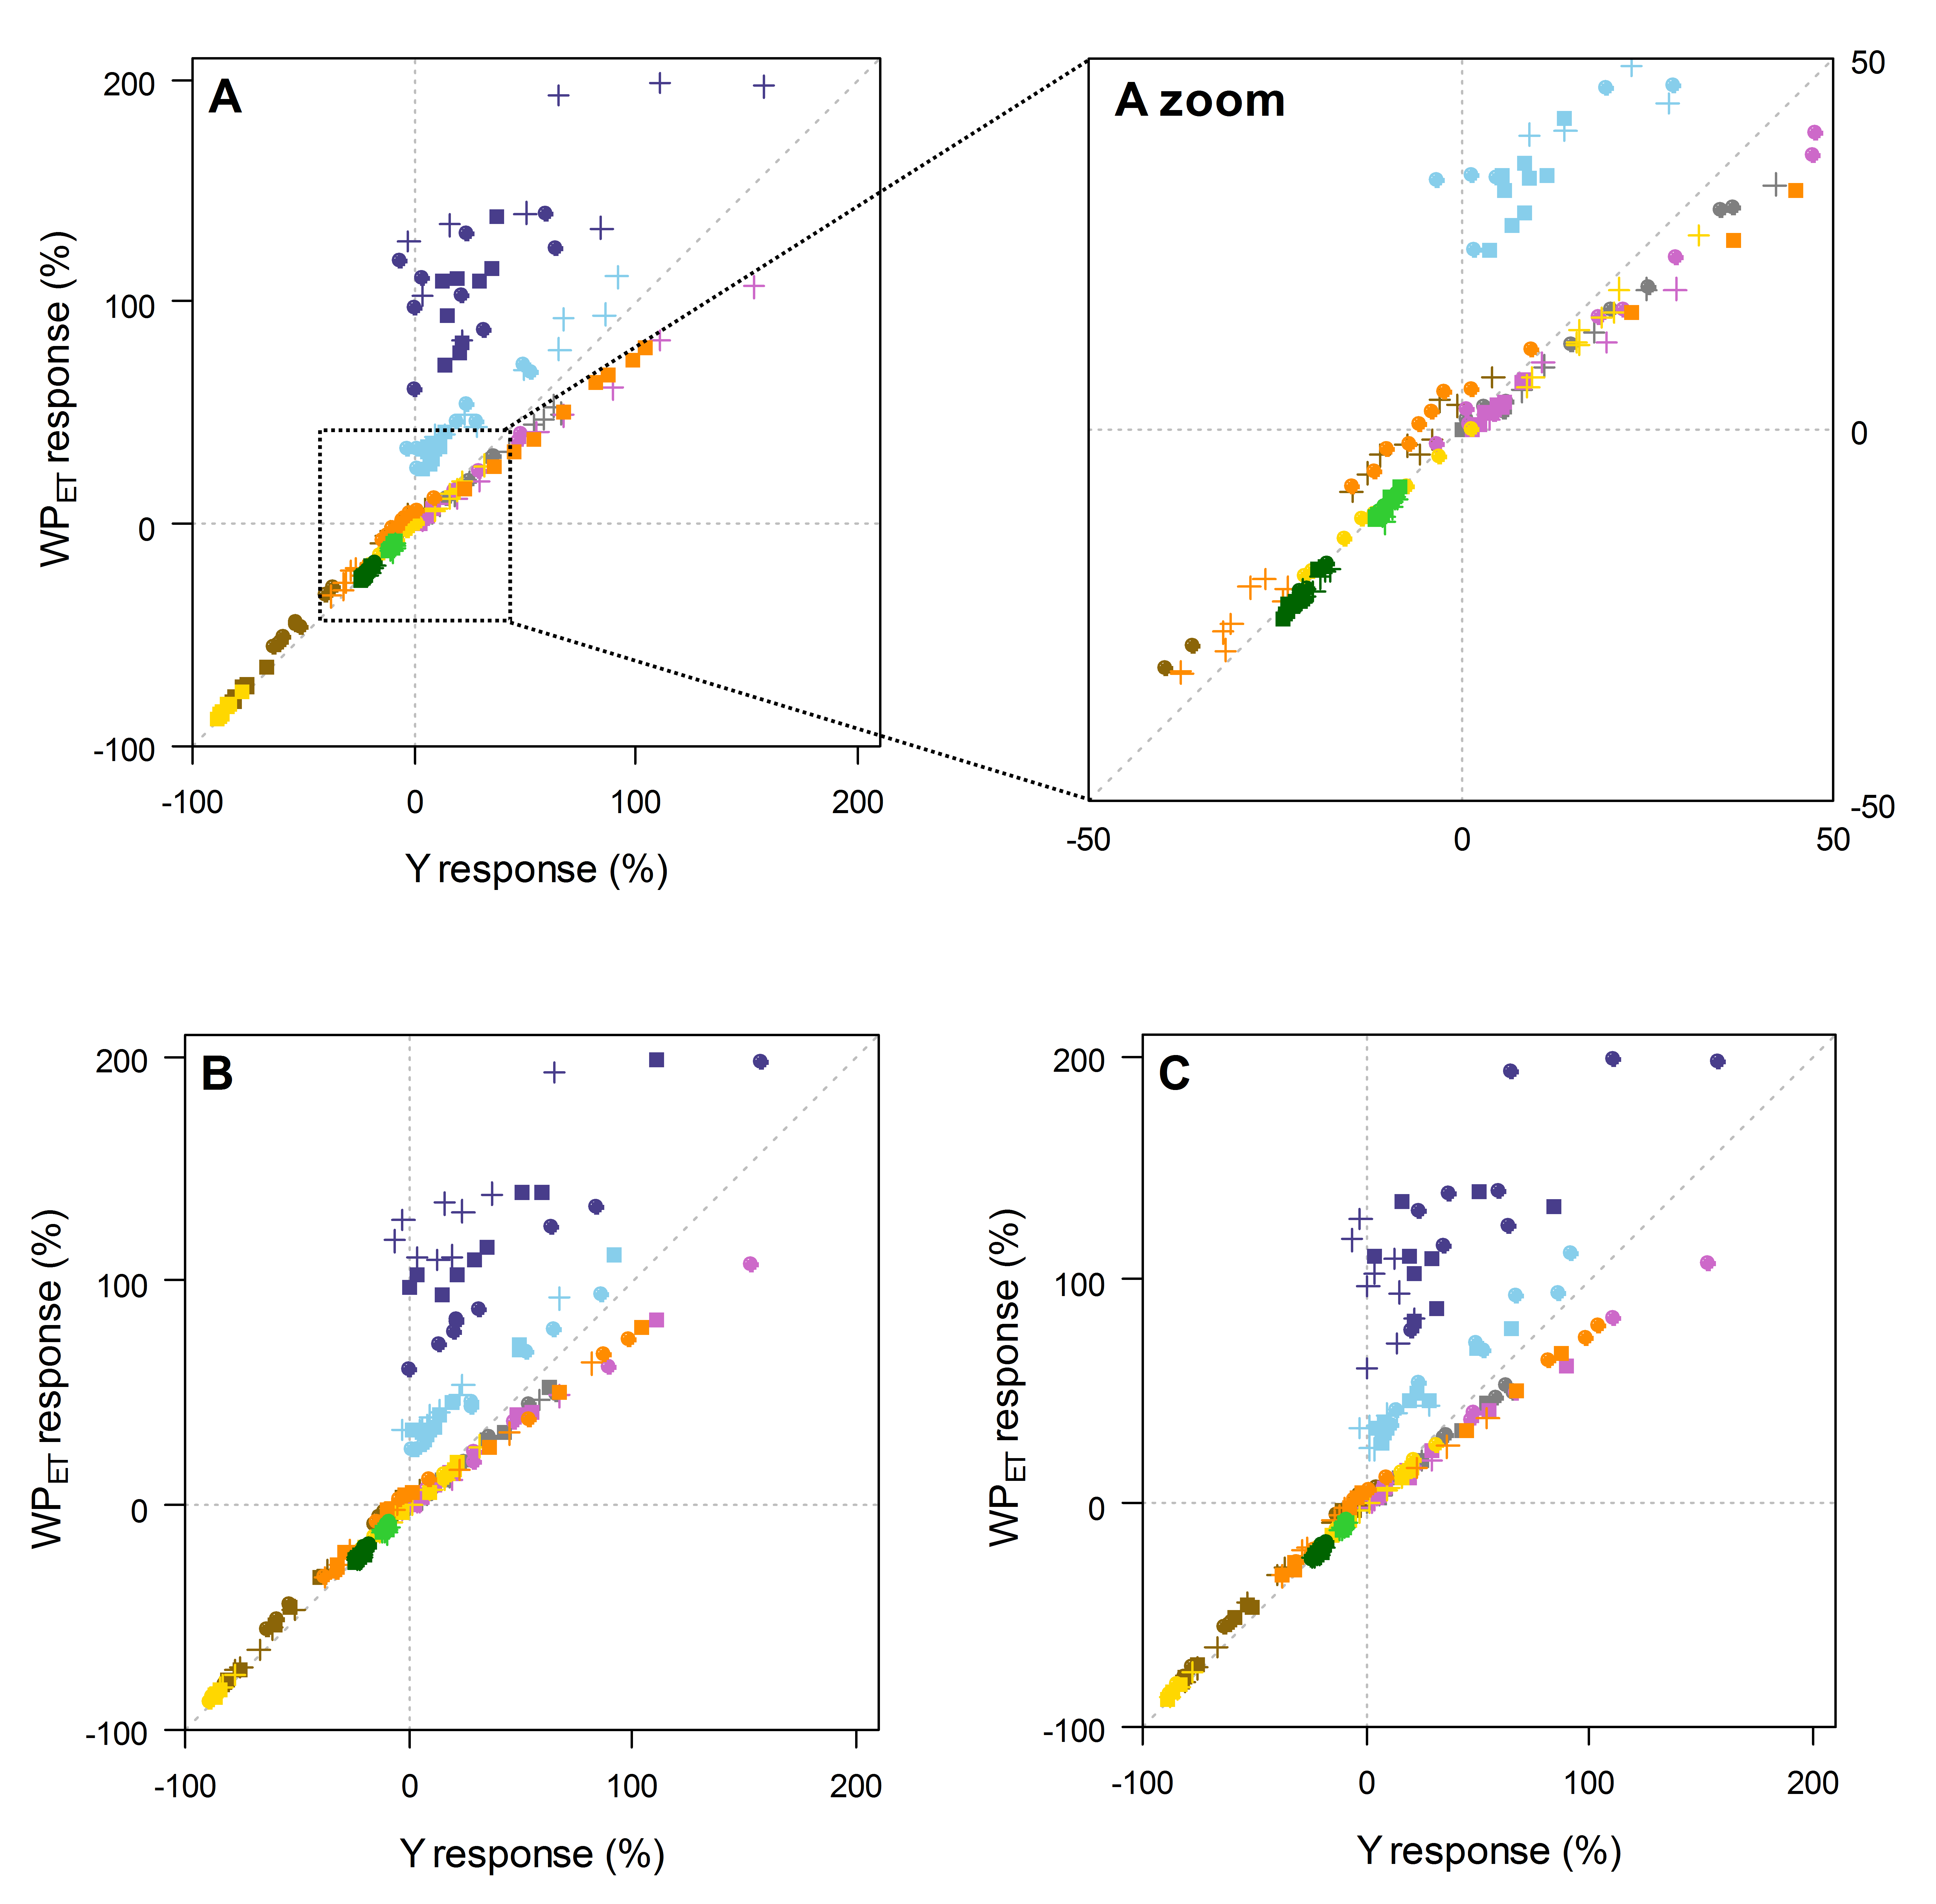
\includegraphics[width=\textwidth]{ScenMekelle_600dpi.png}
		\caption{Average yield (\Y) and crop water productivity (\WPET) response to different agricultural management strategies, i.e. \TAWm (\textcolor{tawm}{$\bullet$}), \TAWp (\textcolor{tawp}{$\bullet$}), Restr (\textcolor{rest}{$\bullet$}), Bunds  (\textcolor{bunds}{$\bullet$}), M50 (\textcolor{m50}{$\bullet$}), M95 (\textcolor{m95}{$\bullet$}), RWH (\textcolor{rwh}{$\bullet$}), W15 (\textcolor{w15}{$\bullet$}), W30 (\textcolor{w30}{$\bullet$}) for normal growing seasons in Mekelle depends on (a) soil type, i.e. clay loam ($\bullet$), loamy sand ($\blacksquare$) and silt ($+$), (b) soil fertility level, i.e. non limiting ($\bullet$), moderate ($\blacksquare$) and poor ($+$), and (c) crop variety with long ($\bullet$), medium ($\blacksquare$) and short ($+$) cycle length.}
	\label{fig:ch5_ScenMekelle}
\end{figure}

\autoref{fig:ch5_ScenMekelle}a clearly indicates that soil types influenced the effect of soil and field surface management. Although the average effect of Restr was negative in normal growing seasons in Mekelle (\autoref{fig:ch5_ScenClim}), the response was much more negative for loamy sand soils compared to clay loam soils. For silt soils the response was sometimes even positive. Also the response to \TAWp and \TAWm clearly followed a pattern related to soil types. For \TAWp the average response was positive (\autoref{fig:ch5_ScenClim}) but that was mainly caused by a positive response on loamy sand soils. On clay loam soils and silt soils the response to \TAWp was even negative. For \TAWm, on the other hand, the response varied from negative for a loamy sand soil to positive for a silt soil. Eventually this resulted in a negative average response (\autoref{fig:ch5_ScenClim}). The fact that silt soils reacted contrary to expectations can be explained by the fact that aeration stress was observed for these simulations. Making the soil reservoir smaller by Restr or \TAWm, relieved part of the aeration stress. Also, the effect of bunds and RWH was soil type dependent. The lower CN value for loamy sand soils (\autoref{tab:ch5_soils}) resulted in lower surface runoff on these soils as compared to other soil types. Consequently, a smaller amount of water could be gained by RWH or bunds, which led to lower responses to those practices on loamy sand soils. 

Next to soil type, \autoref{fig:ch5_ScenMekelle}b shows that also the soil fertility level influenced the effectiveness of management strategies. For example, the \Y response to mulch was smaller on poorly fertilized soils than on soils with non limiting soil fertility. Reducing evaporation with mulches might not be very effective on poorly fertilized soils because soil fertility limits crop production more than water availability. By contrast, the \WPET response to mulches was stronger for poorly fertilized soils than for well fertilized soils. Since crop canopy development was less strong on poorly fertilized soils, also transpiration was lower and evaporation higher than on fields with non limiting soil fertility. For that reason, techniques that reduce evaporation such as mulches had a stronger \WPET response for poorly fertilized soils. 

Furthermore, the response to mulches was also dependent on the crop variety as shown in \autoref{fig:ch5_ScenMekelle}c. \Y response was smaller for crops with a short growing cycle than for crops with a long cycle. Crops with a short cycle experience less water stress because their crop cycle extends less far in the dry season. As such these short cycle varieties crops benefit less from additional soil water in the root zone due to mulches.

\autoref{fig:ch5_ScenClim} and \autoref{fig:ch5_ScenMekelle} indicate which strategies could improve average \Y and \WPET under different environmental conditions. Additional analysis of the effect of agricultural management on the frequency of harvest failure (\autoref{fig:ch5_Failure}) revealed, for example, that for dry seasons in Mekelle the water saving practices that were most beneficial for \Y and \WPET (bunds, RWH, M50, M95, \autoref{fig:ch5_ScenClim}) also decreased the occurrence of harvest failure. Inadequate weed management, on the other hand, decreased \Y and \WPET substantially, but did not affect the occurrence of crop failure. In addition, it is clear from \autoref{fig:ch5_Failure} that the effect of management on the frequency of harvest failure is highly dependent on the soil type of the cropping system. 

\begin{figure}[tbhp]
	\centering
		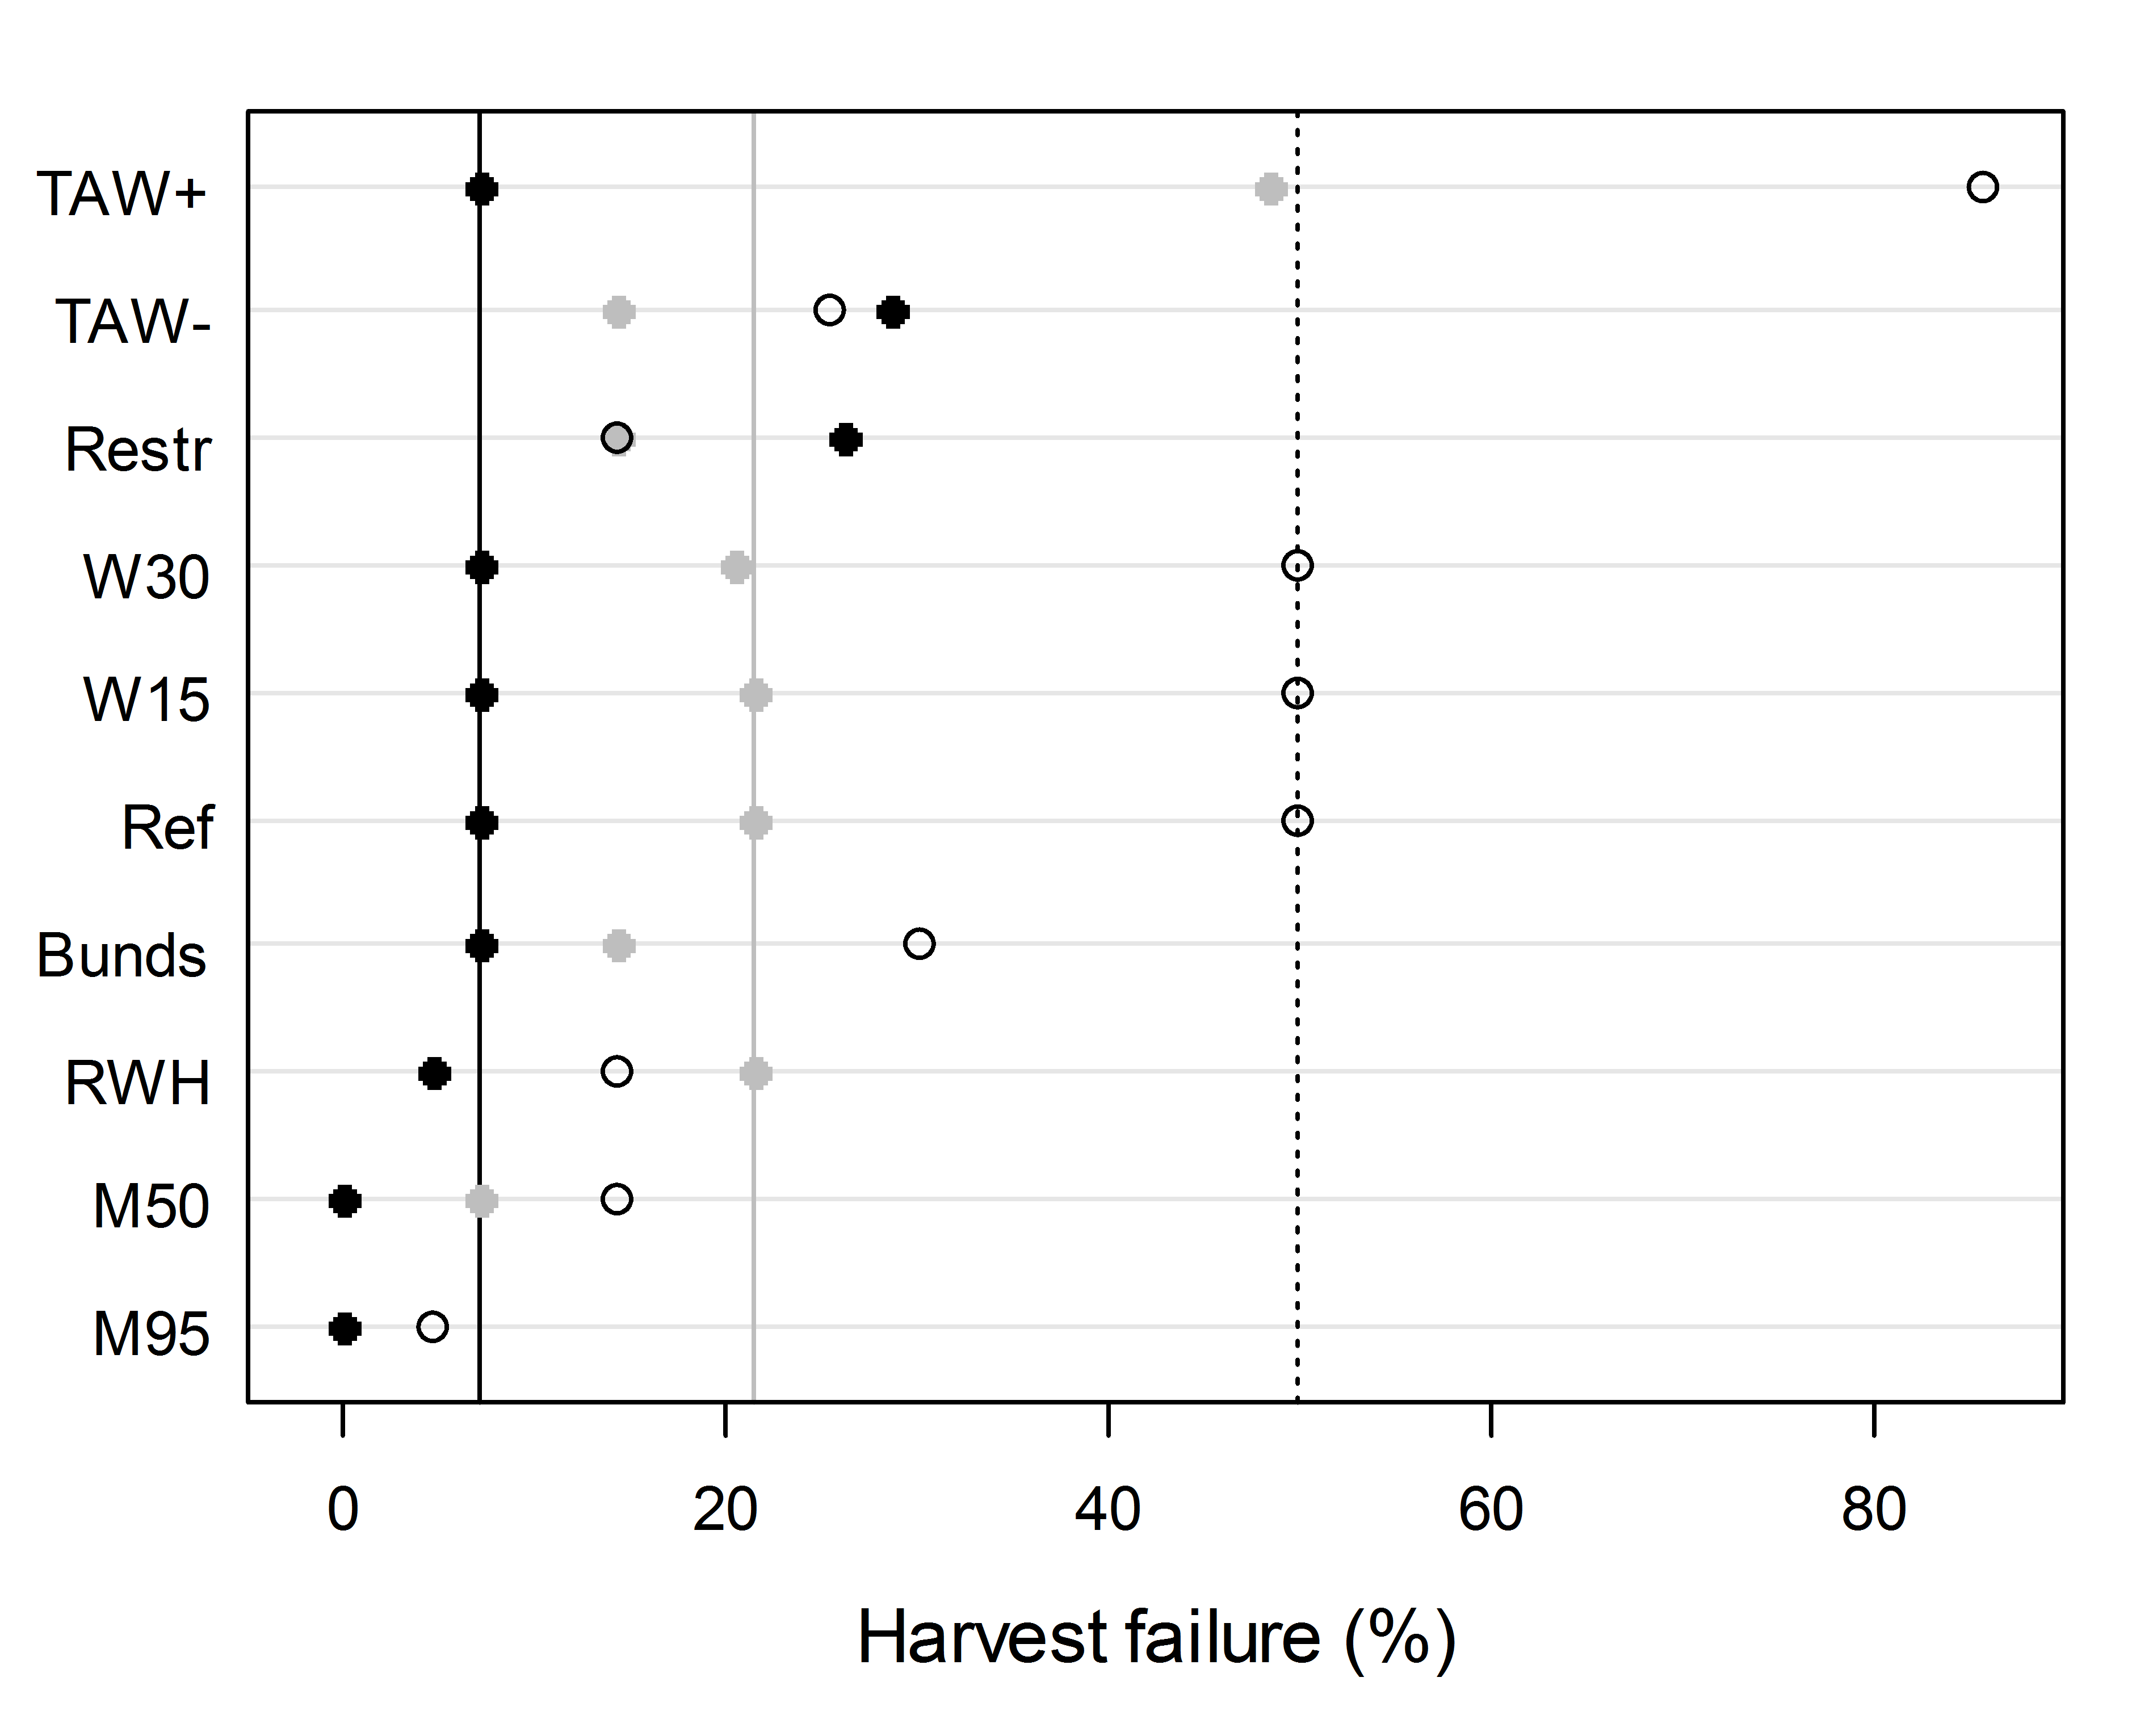
\includegraphics[width=8.5cm]{Failure_600dpi.png}
	\caption{The average percentage of the dry growing seasons in Mekelle with complete harvest failure ($Y=\SI{0}{t/ha}$) on clay loam (\textcolor{bunds}{$\bullet$}), loamy sand ($\bullet$) and silt ($\circ$) soils for different agricultural management strategies. The failure percentage for reference management on each soil type is marked with a vertical line.}
	\label{fig:ch5_Failure}
\end{figure}

\section{Discussion} 
This study illustrated the AquaCrop-based simulation approach to investigate the effectiveness of different agricultural management practices to upgrade (water) productivity for rainfed cropping systems. Hence, it was by no means intended to present the optimal management strategies for the simulated regions, nor to present exact responses that can be expected in farmers' fields. The presented response values are merely indicative and serve as a starting point to compare the effect of various management practices and to explore management-environment interactions.

The proposed simulation approach supports development of agricultural management guidelines that promote a sustainable increase of agricultural productivity. This is due to the fact that the AquaCrop-based approach allows assessment of both \Y and \WPET response to agricultural management. Since water is or is becoming a bottleneck for increasing agricultural production in many regions of the world, the \WPET response to agricultural management is as important as the \Y response. In very dry regions one can even consider implementing management practices that increase \WPET while the effect on \Y is insignificant or slightly negative. In addition, the simulation approach promotes sustainable management practices because management-environment interactions are explicitly accounted for. The presented scenario analysis for drought-prone rainfed farming systems confirmed that the effect of management strongly depends on the environmental conditions. Due to the strong interaction between management, crop, soil and climate, it is crucial that agricultural management strategies are tailored to the local weather conditions, environment and farming system to get the highest \Y and \WPET benefits. Furthermore, consideration of the management-environment interactions, makes that the effect of environmental changes on the effectiveness of agricultural management can be considered in the analysis. For example, the effect of climate change on the effectiveness of agricultural management practices could be investigated, although not illustrated for the presented scenario analysis. This could indicate whether agricultural management practices that are effective under current environmental conditions will remain effective in the future as well. A good example was set by \textcite{lehmann2013} who studied the impact of different climate change scenarios on optimal fertility and irrigation management using CropSyst in combination with an economic decision model.

Furthermore, even though management decisions are to be customized for each cropping system, the AquaCrop simulation approach is applicable for scenario analysis and development of management guidelines on a large spatial scale. For that purpose AquaCrop can be implemented in a GIS environment following the example of \textcite{lorite2013} with AquaGIs or \textcite{thorp2013} with the GeoSim toolbox. In that manner, spatial differences in environmental conditions can be easily linked to spatial differences in productivity and effectiveness of management practices. Furthermore, strategic decisions regarding agricultural management require analysis of their effect in multiple growing seasons. Therefore, simulations should be conducted for a long time series of (historical) weather data. As demonstrated by this study, such a scenario analysis over many growing seasons allows to study the interaction between management and weather conditions, as well as the effect of agricultural management on inter-annual \Y and \WPET variability. Running AquaCrop simulations for large spatial or time scales is facilitated by the use of the user-friendly interface and project modus of AquaCrop, as well as the small computation times of the model. The later can be further optimized by using the AquaCrop plugin version. In addition, \textcite{lorite2013} developed the AquaData tool to facilitate input and output data processing for extensive AquaCrop simulation studies. 

The presented simulation approach has some limitations which affect results and consequently need consideration when using the approach to develop management guidelines. First, it is important to note that the presented scenario analysis was purely based on model simulations without any field validation. Ideally, field observations of soil characteristics, crop characteristics, crop development and production should be collected to complement the simulations. On the one hand, such field observations can serve to calibrate the AquaCrop model parameters to match the local farming conditions in order to improve the accuracy of simulation results. On the other hand, field observations can be used to validate simulation  results. In addition, field experiments can also complement the simulation approach by testing management practices with high potential under realistic agronomic conditions in farmer's fields.

Moreover, the presented simulation AquaCrop-based approach is affected by limitations of the AquaCrop model itself. Scenario analysis is confined to the management practices implemented in AquaCrop. Though extensive options are available as discussed in \autoref{sec:ch2_Mgmt}, some management practices such as disease control and intercropping can not be simulated using AquaCrop. Furthermore, some of the calculation procedures for agricultural management, implemented in AquaCrop 4.0*, need to be adjusted. The presented scenario analysis showed that the simulated effect of practices affecting the soil water holding capacity (\TAWm, \TAWp and Rest) was sometimes counter-intuitive. These unexpected results are most likely caused by the fact that AquaCrop evaluates water stress by evaluating the soil water content over the complete root zone, without taking into account neither water nor root distribution within the soil profile. For example, AquaCrop might simulate the presence of water stress when only the topsoil is wet and the rest of the root zone is dry. In reality, a crop might not suffer from water stress since the majority of roots is located in the topsoil where sufficient water is available. Hence, a future update of the AquaCrop water stress calculation procedures seems necessary to improve simulation of crop responses to water stress and the way that these responses are influenced by agricultural management. Next, the simulated \Y and \WPET decline due to the presence of a restrictive soil layer is most likely overestimated. In the AquaCrop simulation procedure, a restrictive layer completely stops root development, while in reality such a layer would only slow down root expansion. Since some roots can reach deeper soil layers and extract water despite the presence of a restrictive layer, the crop is less vulnerable to water stress than what is simulated by AquaCrop. Moreover, the presented scenario analysis showed that the effect of weed management was almost independent of the environmental conditions of the cropping system. Clearly, the weed management procedure as implemented in AquaCrop 4.0$^\ast$ did not accurately capture the weed-environment interactions and needs to be revised. As presented in \autoref{ch:weed} such a new weed management procedure has been developed and implemented in AquaCrop 5.0*.
 
Furthermore, evalation and comparison of various management strategies in the presented scenario analysis completely relied on assessment of average \Y and \WPET response values. However, one should take care when disregarding the absolute \Y and \WPET numbers. Also, \textcite{rockstrom2007b} mention that \Y and \WPET responses to agricultural management are potentially higher when the absolute reference \Y is low. Increasing \Y from a level that is already substantially high, on the other hand, does not necessarily lead to large \WPET responses. Moreover, next to the average \Y and \WPET levels, it is crucial to assess inter-annual productivity variability. In this study yield variability was only briefly touched upon by evaluation of the harvest failure frequency. More detailed analysis of the complete distribution of \Y and \WPET under various management strategies and environmental conditions could be done by means of cumulative probability density functions, or summarizing statistics such as the coefficient of variation. 

Although the proposed modelling approach provides very valuable insights to optimize agricultural management, this approach can not stand by itself. Research results need to be placed in a broader context and further evaluated with respect to the institutional and socio-economic factors that determine successful adoption and implementation of the proposed management practices.
For example, while this study demonstrated the strong interaction between seasonal rainfall and effectiveness of the various management strategies, farmers are unable to control weather conditions nor to adapt management to the expected rainfall every season. Risk-averse behavior makes that smallholder farmers mostly prefer practices that optimize productivity and limit harvest failure in the dry seasons if crop production is already satisfactory in normal and wet years \parencite{kijne2009}. Hence, the high potential strategies that are indentified with the simulation approach, should be further evaluated from an institutional and socio-economic point of view. To evaluate the economic feasibility of certain practices, the presented simulation approach could be extended by linking AquaCrop to an economic model. Examples have been presented by \textcite{garciavila2009}, \textcite{garciavila2012} and \textcite{cusicanqui2013} who used a combination of AquaCrop and an economic model to optimize irrigation management. Furthermore, the off-site effects of agricultural management need to be evaluated before being implemented. While certain practices might increase water availability at field scale, they might be detrimental for water availability in the region. To investigate both the on-site and off-site effects of agricultural management, AquaCrop could be linked to hydrological models as demonstrated in the following chapters (\autoref{ch:aquacrophydro} and \autoref{ch:achtoep}).
\clearpage
\section{Conclusion}
The AquaCrop-based simulation approach presented and illustrated in this study is a practical and powerful tool to evaluate a broad range of agricultural management strategies for upgrading crop (water) productivity in drought-prone rainfed cropping systems, and to tailor these management strategies to the local agronomic and environmental conditions. The key advantage of this approach is that the effect of various agricultural management practices can be studied on grain yield and crop water productivity at the same time. This makes the approach very suitable for regions where water availability is limited or is likely to become a bottleneck for increasing agricultural productivity. Moreover, the simulation approach can account for the complex interactions between management, soil properties, crop characteristics, and current or future climatic conditions. Finally, also the wide-ranging applicability, the user-friendly software interface and small computation times, together with the ability to combine the model with additional tools make AquaCrop an excellent tool for extensive agricultural management scenario analysis.

\cleardoublepage